
\documentclass{article}
\usepackage[utf8]{inputenc}
\usepackage{graphicx}
\title{EPI-USE: IoT-Homecare \\
The Inevitables
}

\author{  
            Peter Rayner\\
            Dawie Pritchard\\
            Drew Langley\\
            Riaan van der Merwe\\
            Lyle Nel\\
        }


\begin{document}

\maketitle

\newpage

\tableofcontents

\newpage


\section{High level description}
A high level description of the project including the technologies you would like to
use to address the project needs. Illustrate with a deployment diagram.

A home care system that takes advantage of the Internet of Things. The system will make use of existing devices and sensors to deliver a holistic system for monitoring homecare patients.
The system will gather details from a patient from the devices and sensors and communicate them in a generic manner using Wi-Fi with the caregivers through a mobile application and EPI-USE's cloud server (EPIUSE pdf.2017)

Technologies we would like to use.
J2EE
JDBC
JPA
wildfly 10
GlassFish 4
Using a microservices architecture where each microservice can be managed, developed and released independently\\
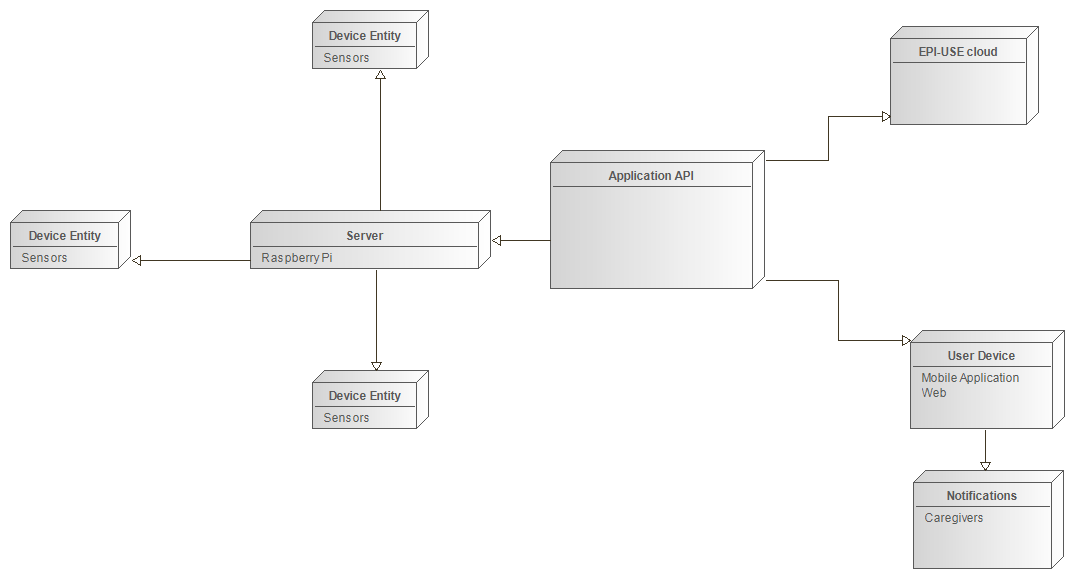
\includegraphics[width=\linewidth]{dd.png}
As seen this architecture promotes loose coupling and high cohesion that is required to implement the API.

\section{development methodology}

We will be using the Scrum methodology. By making a backlog of work to be done, by completing deadlines in short iterations or sprints. We will meet daily on the slack group to describe progress as well as obstacles and overcome these obstacles by getting input from each member. We will also define when these deadlines are and make sure we keep checking to make sure we dont fall behind. We will meet everytime we are done with a deadline to reflect on the work done.
At each deadline or meeting we will make sure we meet with the client to make sure he knows we are making progress. We will also meet when there are concerns or obstacles to overcome to make sure the client knows full well about these obstacles. The client will be kept up to date each week with the progress of the project.

\section{Team details}
Dawie Pritchard: \\Multimedia Specialist, Computer Scientist\\
Technologies known\\ C++,C-Sharp,C,Java,Python,AngularJS,ExpressJS,NodeJS,MongoDB,Php,SQL\\,NOSQL,HTML5,CSS,Bootstrap,JQUERY,Javascript,XML\\
Other skills:\\ Human Computer Interaction, Trends, Visual Design \\
Stengths: \\Front-End, Back-End development

\end{document}